\section{Introduction}
%\section and \subsection are included in the table of contents

\subsection{Background}
%J'ai pas mal de peine à ecrire l'introduction so I'm hoping once we continue writing qu'on arrive à voir mieux ce qu'il faut enlever ajouter à l'intro. Enfaite dépendant de comment on veut struturer notre texte je metterais ou enleverais des informations

Authentication entails confirming the validity of a claimed identity seeking access to a system or resource. Over decades, authentication mechanisms have evolved from basic password systems in the 1960s to advanced methods such as multifactor authentication by the late 2010s, driven by a persistent commitment to combat evolving security risks while enhancing user convenience\footnote{\url{https://cybersecurity.asee.io/blog/history-of-authentication/}}. Various methods such as password-based authentication, certificate-based authentication, one-time passwords multifactor authentication, and biometric authentication are employed\footnote{\url{https://www.microsoft.com/en-us/security/businesssecurity-101what-is-authentication.}}. Biometric authentication, which involves analyzing unique physical characteristics, is often considered more secure than traditional authentication methods due to the difficulty in duplicating biometric traits. This encompasses technologies such as facial recognition, fingerprint recognition, eye recognition, and voice recognition\footnote{Problem with url}. %\url{https://www.logintc.com/types-of-authentication/biometric-authentication/#:~:text=Biometric%20authentication%20refers%20to%20a,%2C%20retinas%2C%20and%20facial%20features}  
\newline However, despite the enhanced security of biometric authentication, it is not immune to exploitation. For instance, fingerprints left on surfaces can be copied, or hackers may obtain images of individuals online to deceive authentication systems. 

While advanced biometric systems typically rely on externally visible physical attributes, finger-vein authentication focuses on internal anatomical features, adding a unique layer of security, as they are less prone to replication or theft compared to external characteristics. Nevertheless, it is important to note that finger-vein authentication does not completely eliminate challenges. Despite its emphasis on internal features, attackers can exploit inherent structures in finger veins, such as common patterns among individuals and predictability in acquired data, which poses risks to the authentication process.

%-> Mentionner que biometric should be combined with other security mechanisms?

%-> Si on a des question on peut contacter BioId!
%This project focuses on authentication using finger-vein features, employing a scanner equipped with two infrared cameras to capture finger veins from distrinct angles. These cameras can perform local computations and communicate with a server infrastructure. Upon registration, the captured image referred to as the model image, is encrypted and transmitted to a secure database. During authentication, another image of the finger, known as the probe image, is acquired. Subsequently, either the model or the probe image is transmitted over the network and then realigned to enable computation of a similarity score between them. 
In light of these considerations, this project is dedicated to authentication using finger-vein features.
This involves utilizing a specialized scanner equipped with two infrared cameras to capture finger veins from different angles.
The registration process involves capturing an image, termed the model image, while the authentication process involves capturing another image, known as the probe image. These images undergo processing through a pipeline designed to extract and align the finger-vein patterns. The importance of this pipeline cannot be overstated; it aligns and processes the images to accurately compare the model and probe images.
Ultimately, the pipeline outputs a feature vector, which is essentially a bitstring, where 0's represent where there are no finger veins, and 1's show where veins are present.Following this process, the system evaluates whether the feature vector extracted from the probe image sufficiently matches the feature vector of the model image associated with the individual attempting authentication. This assessment ultimately determines the authentication outcome.



\subsection{Presentation of the Project}

%Explain what we will be testing/implementing in this project without getting into too many details yet (we will get more in detail in the theoretical framework where we explain what is in the fuzzy hash sections 1-5 and how we will test what is in there)
%Explain the state of the current project (where is it left, what has been achieved already, by both Burcu and Simon)
%Briefly introduce the concept of fuzzy hashing (security reasons and usability)

This project extends the work on optimizing a finger-vein recognition pipeline that has demonstrated the lowest Equal Error Rate (EER) \hyperref[def:EER]{Equal Error Rate (EER)} by incorporating a novel hashing step to process the output. The purpose of integrating \hyperref[def:Hash_Function]{hash functions} within this context is twofold: to bolster the security of biometric data by converting it into a hash value, hence safeguarding against unauthorized reconstruction of the biometric template, and to enhance the system's efficiency by facilitating rapid comparison of hashed values in place of actual biometric data. But before going into hash functions, being the heart of our project, we would like to start by presenting the state that the project was in when we started building on top of it.

Simon Sommerhalder and Burcu Yildiz have both made significant contributions to the system. Simon has developped a pipeline (see Figure~\ref{simon_pipeline}) to align finger-vein images independently, enhancing security by eliminating the need to compare the model and probe images side by side. He organized the process into six clear steps:

\begin{enumerate}
    \item \textbf{Masking}: The first step of the pipeline isolates the finger area in the image. This involves creating a mask that outlines the finger, ensuring that subsequent processing focuses solely on the relevant part of the image.

    \item \textbf{Prealignment}: This step involves adjusting the position and orientation of the finger within the image before extracting vein patterns. It's aimed at roughly aligning the image based on the finger's outline, helping to standardize the position of the finger across different scans.

    \item \textbf{Histogram equalization}: To ensure the images have consistent lighting and contrast, this step adjusts the brightness levels. This makes the vein patterns more distinct and comparable across different images.

    \item \textbf{Feature extraction}: Here, the actual vein patterns are identified and extracted from the image. The process converts the visual image into a digital format that represents the presence or absence of veins at specific locations.

    \item \textbf{Postalignment}: After extracting the vein patterns, this step fine-tunes the alignment of the image. It's based on the vein patterns themselves, ensuring that the comparison between model and probe images is as accurate as possible.

    \item \textbf{Distance Caclulation}: The final step involves comparing the feature vector of the probe image with that of the model image. This is done using a specific metric to quantify the similarity between the two, ultimately determining if they match closely enough for authentication to succeed.
\end{enumerate}

This organization allows each part of the process to be individually assessed and improved. Additionally, Simon has developed various functions to boost the system's efficiency and achieve the optimal balance between false acceptances and rejections. 

\begin{figure}[!h]
    \centering
    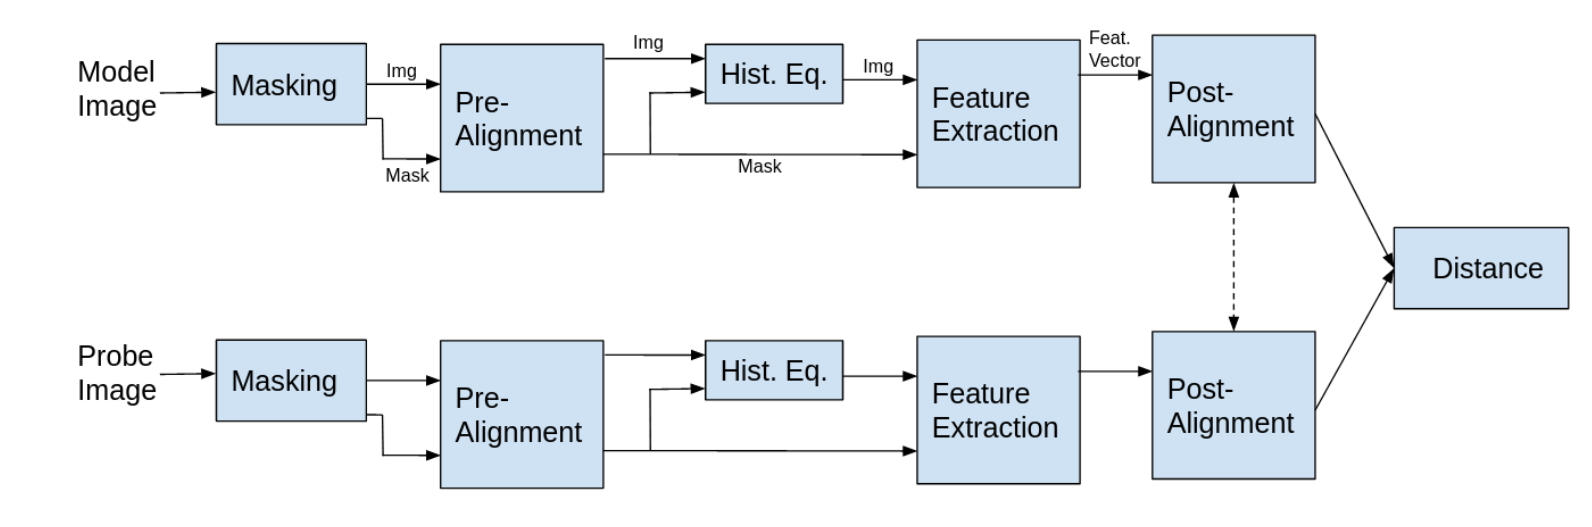
\includegraphics[width=1\linewidth]{latex-img/pipeline_simon.png}
    \caption{Simon's Extraction Pipeline. Compares a single probe image to a model image}
    \label{pipeline_simon}
\end{figure}


%\subsection{Structure of the Report}
%Explain how our report will be structured -> Explain how we needed to start by understanding and retesting (as asked from Serge) what had been done before us (the software part as we have already covered what has been done on a high level in the introduction). We also needed to assess again the efficiency of the algorithms developped by Simon and Burcu. Then, explain that we will start by going through the theoretical concepts that we need to understand in order to implement everything (sections 1-5 from fuzzyhash). Then we will move onto the actual software implementation, 1:N matching (etc...) -> on doit update ceci à la fin et expliquer ce qu'on a actually réussi à faire


%Additional comments and definitions (may or may not be useful)
%Fuzzy Hashing: Fuzzy hashing is a technique used to generate a hash value that remains consistent even when the input data has minor variations. This is particularly useful in biometrics, when the data captured(like finger-vein patterns) may have slight differences each time due to changes in the environment or the way the biometric trait is presented.
%Fuzzy hashing: is a technique used to generate hash values for data such that similar inputs produce similar hash values. It is particularly useful in situations where the input data may have minor variations or noise, such as in biometric authentication systems where slight differences in captured biometric data can occur due to environmental factors or variations in how the viometric trait is presented. Fuzzy hashing enables efficient comparison of similar data by mappin it to hash values that are close to each other.

%Purpose of hashing: By storing a hash of the extracted biometric feature rather than the extracted feature itself, the privacy of the user is enhanced. Even if the hash data is compromised, it should not reveal any personal biometric information. Hashed values have fixed sizes which makes storage requirements predictable and efficient. 

%Fuzzy Extractors: takes the concept of fuzzy hashing further by enabling secure error-tolerant biometric authentication. It consists of two main algorithms, Gen (generate) and Rep (reproduce). It enables the secure extraction and reproduction of a key from noisy input data, like biometric data. 